% Iberian Cantilevers -- feature overview
% Build: latexmk -pdf iberian_cantilevers.tex   (or pdflatex twice)
\documentclass[11pt,a4paper]{article}

\usepackage[T1]{fontenc}
\usepackage[utf8]{inputenc}
\usepackage{lmodern}
\usepackage[english]{babel}
\usepackage[margin=2.2cm]{geometry}
\usepackage{graphicx}
\usepackage{caption}
\usepackage{subcaption}
\usepackage{booktabs}
\usepackage{tabularx}
\usepackage{xcolor}
\usepackage{enumitem}
\usepackage{float}
\usepackage[section]{placeins}
\usepackage[hidelinks]{hyperref}

\definecolor{iberianred}{RGB}{150,42,36}
\captionsetup{font=small,labelfont={bf,color=iberianred}}
\setlist{itemsep=2pt,topsep=4pt}
\graphicspath{{img/}}

% figures: fill text pages generously and stack figure-only pages from the top
\renewcommand{\topfraction}{0.9}
\renewcommand{\bottomfraction}{0.8}
\renewcommand{\textfraction}{0.07}
\renewcommand{\floatpagefraction}{0.7}
\makeatletter
\setlength{\@fptop}{0pt}
\setlength{\@fpsep}{12pt plus 1fil}
\setlength{\@fpbot}{0pt plus 1fil}
\makeatother

\newcommand{\photocredit}[1]{\par\vspace{1pt}{\scriptsize\color{gray}#1}}
\newcommand{\shot}[2][\linewidth]{\includegraphics[width=#1]{game/#2}}

\title{\color{iberianred}\textbf{Iberian Cantilevers}\\[4pt]
\large Overhead line equipment from the Iberian Peninsula\\for \emph{Create: Pantographs \& Wires}}
\author{Feature overview}
\date{Minecraft 1.20.1 (Forge) \quad$\cdot$\quad version 0.1.0 \quad$\cdot$\quad October 2026}

\begin{document}

\maketitle

\begin{figure}[H]
  \centering
  \shot{linea_iberica.png}
  \caption{A stretch of line built with the add-on: Iberian lattice masts, Iberian cantilevers in zigzag
  and the overhead wire of \emph{Create: Pantographs \& Wires}.}
\end{figure}

\begin{center}
\small\itshape Developed by a railway enthusiast.
\end{center}

\newpage
\tableofcontents
\vspace{1em}

% ---------------------------------------------------------------------------
\section{Overview}

\textbf{Iberian Cantilevers} is an add-on for \emph{Create: Pantographs \& Wires} (PNW) that adds overhead
line equipment as it is built on the railways of the Iberian Peninsula, mostly following Spanish practice:
the cantilevers (\emph{m\'ensulas}) of the conventional network, the masts that carry them, the rigid
overhead conductor rail used in tunnels and an Iberian-style pantograph.

The add-on does not replace any part of PNW. It plugs into PNW's wire system: its blocks are PNW wire
connectors, the catenary wire of PNW is strung onto them as usual, pantographs collect current from them in
the same way, and the masts share PNW's tags, so PNW blocks and Iberian blocks can be mixed freely on the
same line.

\paragraph{Contents of the add-on}
\begin{itemize}
  \item \textbf{Iberian Cantilever} -- a configurable cantilever modelled on the Spanish one, with three
        zigzag positions, three insulator types and an optional support wire (Section~\ref{sec:cantilever}).
  \item \textbf{Iberian masts} -- flat lattice (straight and diagonal) and square lattice masts with four
        weathering stages and waxing (Section~\ref{sec:masts}).
  \item \textbf{Rigid catenary} -- an overhead conductor rail strung like a wire, which follows curves and
        can be joined to the flexible catenary (Section~\ref{sec:rigid}).
  \item \textbf{Iberian Tunnel Support} -- ceiling and wall supports for the rigid catenary in several sizes
        (Section~\ref{sec:tunnel}).
  \item \textbf{Iberian Pantograph} -- PNW's pantograph with the red frame typical of Iberian trains
        (Section~\ref{sec:pantograph}).
\end{itemize}

% ---------------------------------------------------------------------------
\section{Real-world reference}

On the Spanish conventional network the contact wire is usually held by \emph{cantilevers}: a steel tube
fixed to a lattice or H-beam mast, which rises in a short diagonal and then runs horizontally over the track.
The messenger wire rests on an insulator on top of the tube, and a registration arm hanging from the
cantilever pulls the contact wire alternately to each side of the track (\emph{zigzag}), so that the
pantograph strip wears evenly. A support wire (stay) often runs from the mast to the elbow of the tube.

\begin{figure}[htbp]
  \centering
  \begin{subfigure}[t]{0.49\linewidth}
    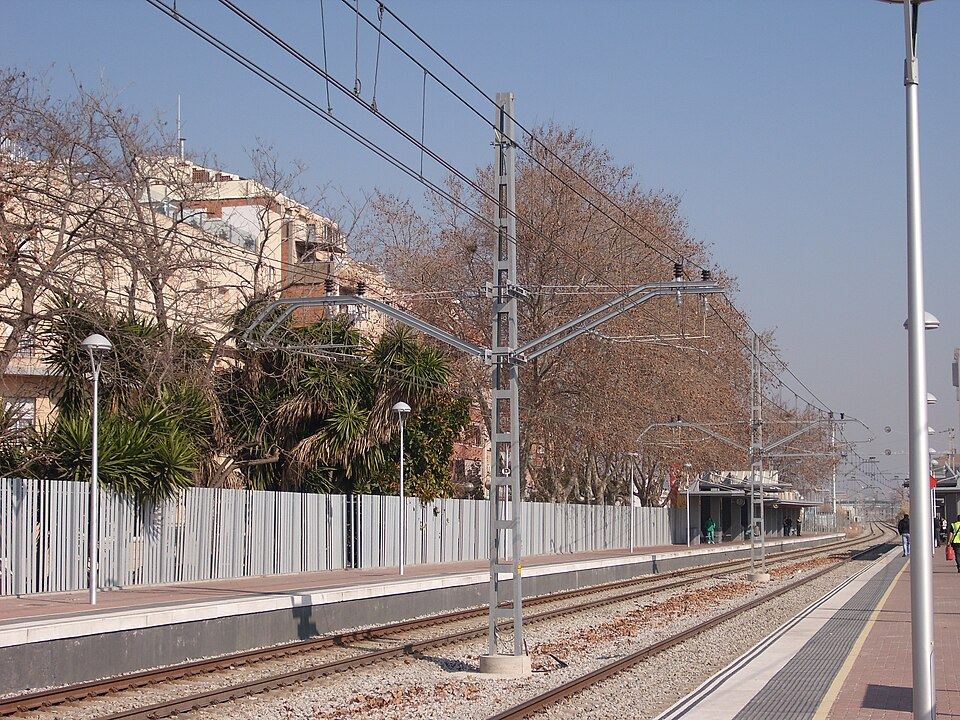
\includegraphics[width=\linewidth]{photos/sant_adria.jpg}
    \caption{Cantilevers on lattice masts, Sant Adri\`a de Bes\`os.}
    \photocredit{Adif -- Ineco, CC BY-SA 3.0, via Wikimedia Commons.}
  \end{subfigure}\hfill
  \begin{subfigure}[t]{0.49\linewidth}
    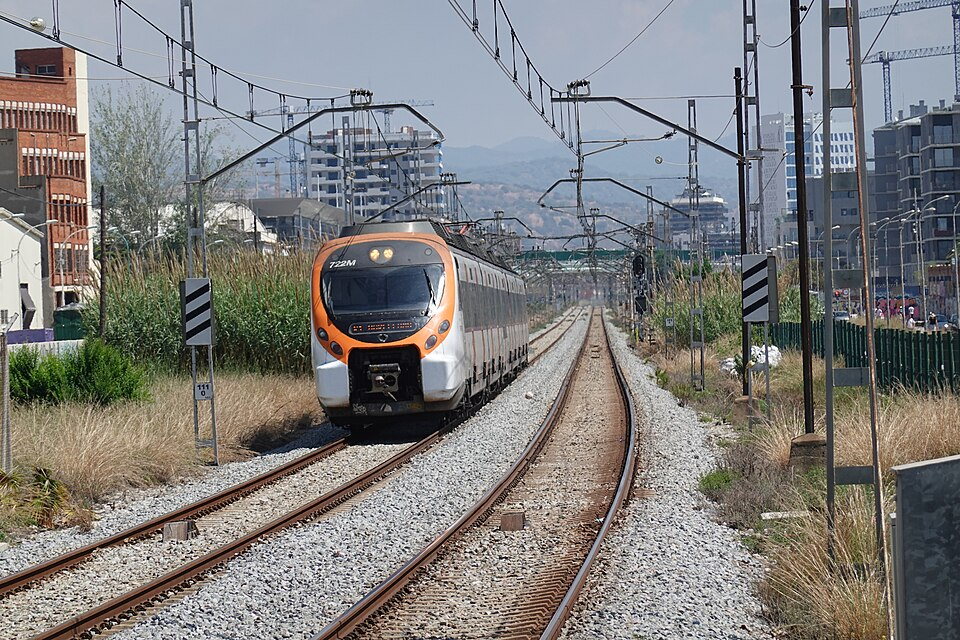
\includegraphics[width=\linewidth]{photos/sant_adria_rodalies.jpg}
    \caption{Commuter train under cantilevers on lattice masts, Sant Adri\`a de Bes\`os.}
    \photocredit{Smiley.toerist, CC BY-SA 4.0, via Wikimedia Commons.}
  \end{subfigure}
  \caption{Cantilevers of the Spanish conventional (Iberian gauge) network.}
\end{figure}

\begin{figure}[htbp]
  \centering
  \begin{subfigure}[t]{0.49\linewidth}
    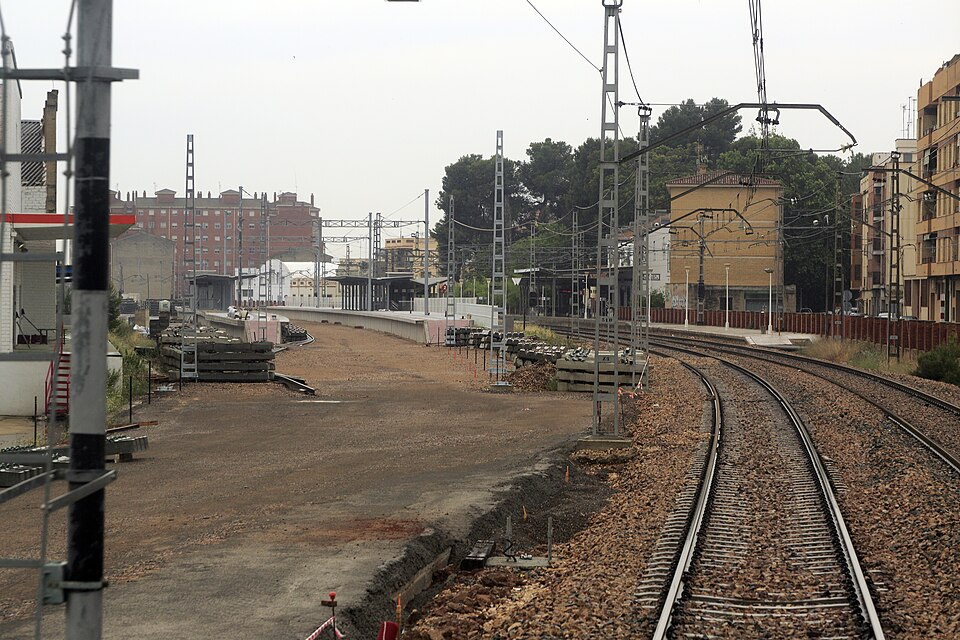
\includegraphics[width=\linewidth]{photos/nules.jpg}
    \caption{Conventional line with cantilevers on lattice masts, Nules (Valencia--Castell\'on).}
    \photocredit{Falk2, CC BY-SA 4.0, via Wikimedia Commons.}
  \end{subfigure}\hfill
  \begin{subfigure}[t]{0.49\linewidth}
    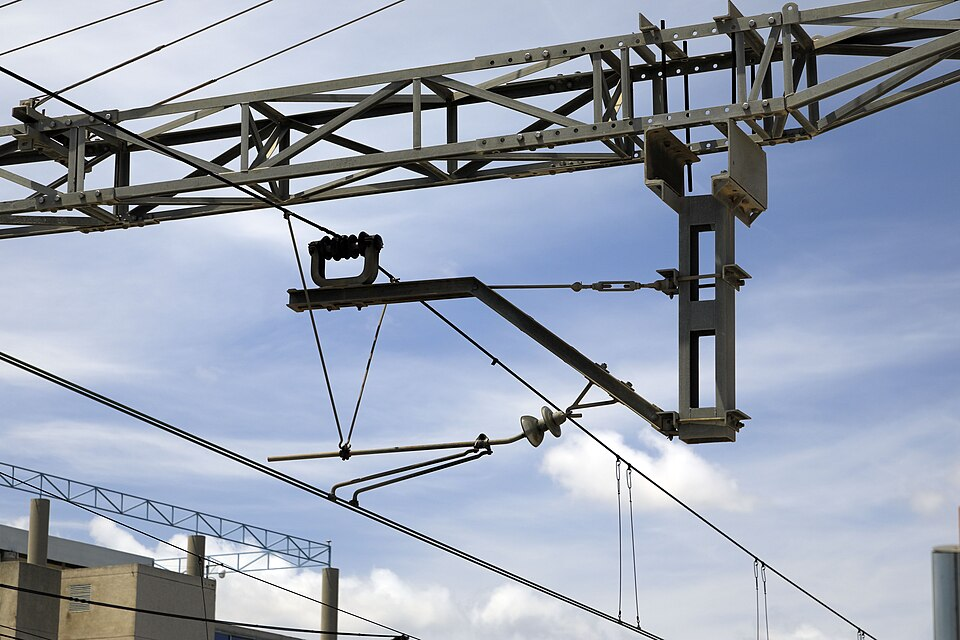
\includegraphics[width=\linewidth]{photos/valencia_registration_arm.jpg}
    \caption{Detail of a cantilever with its insulators and registration arm, Val\`encia Font de Sant Llu\'is.}
    \photocredit{Falk2, CC BY-SA 4.0, via Wikimedia Commons.}
  \end{subfigure}
  \caption{Conventional catenary in the Valencia area.}
\end{figure}

In tunnels and underground stations the flexible catenary is often replaced by a \emph{rigid catenary}:
an aluminium or steel profile that clamps the contact wire and hangs from short supports fixed to the
ceiling or to the tunnel wall. It needs very little height and almost no maintenance of tension.

\begin{figure}[htbp]
  \centering
  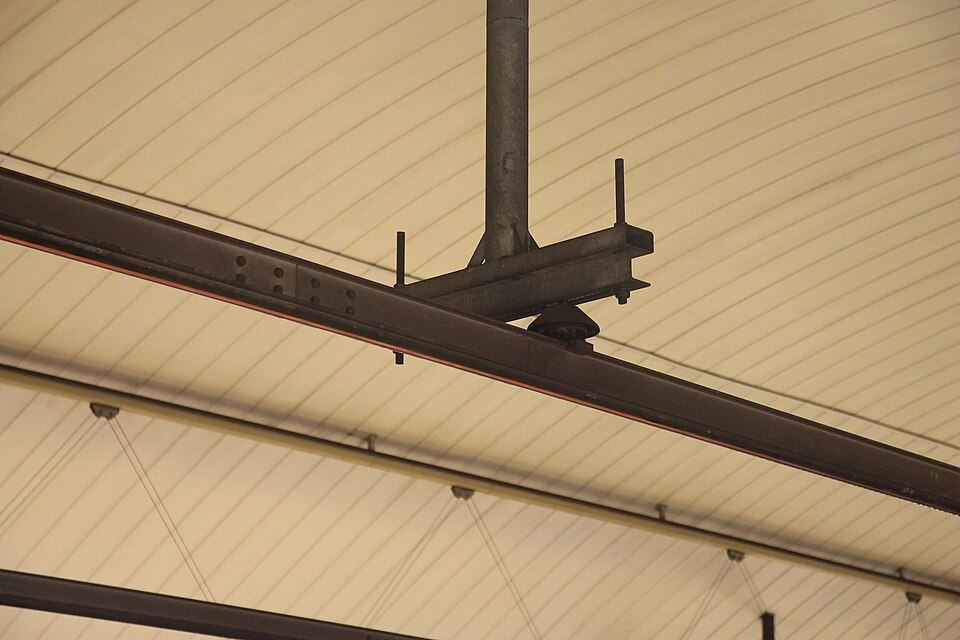
\includegraphics[width=0.7\linewidth]{photos/rigid_nuevos_ministerios.jpg}
  \caption{Rigid catenary and its ceiling supports, Nuevos Ministerios (Madrid Metro, Line 10).}
  \photocredit{Draceane, CC BY-SA 4.0, via Wikimedia Commons.}
\end{figure}

Many Spanish electric trains carry pantographs with a frame painted red, which is where the colour of the
Iberian Pantograph comes from.

\begin{figure}[htbp]
  \centering
  \begin{subfigure}[t]{0.49\linewidth}
    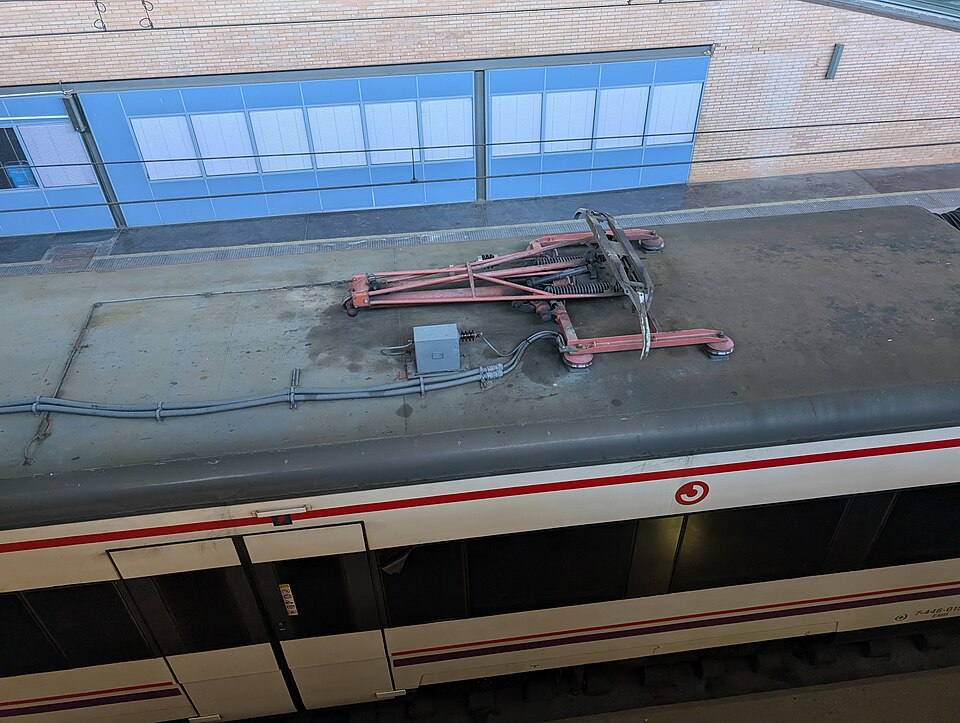
\includegraphics[width=\linewidth]{photos/pantograph_446.jpg}
    \caption{Pantograph on a Renfe Class 446 train, C\'ordoba.}
    \photocredit{Philip Mallis, CC BY-SA 4.0, via Wikimedia Commons.}
  \end{subfigure}\hfill
  \begin{subfigure}[t]{0.49\linewidth}
    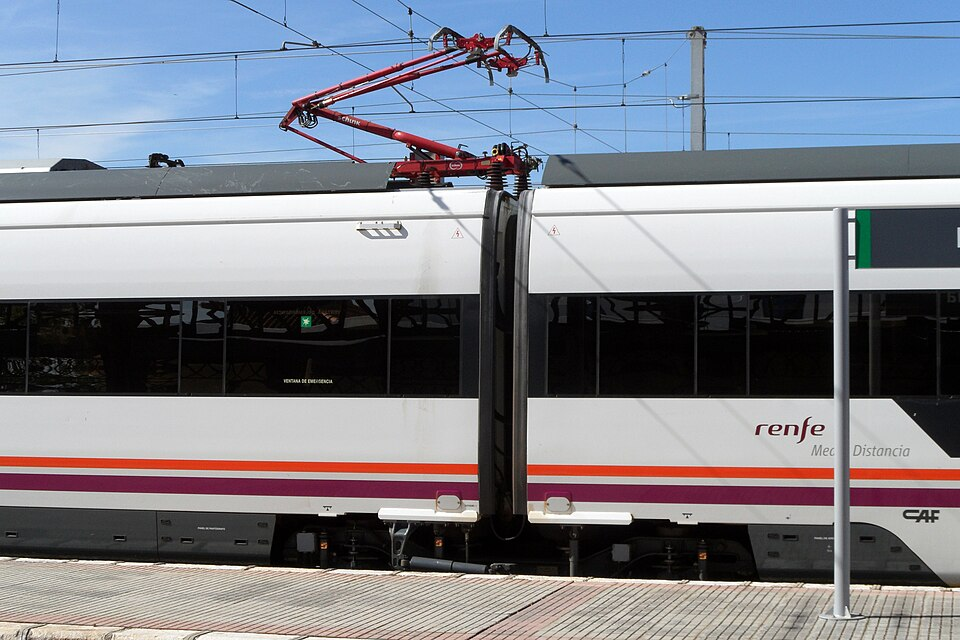
\includegraphics[width=\linewidth]{photos/pantograph_449.jpg}
    \caption{Pantograph on a Renfe Class 449 train.}
    \photocredit{Falk2, CC BY-SA 4.0, via Wikimedia Commons.}
  \end{subfigure}
  \caption{Red pantograph frames on Spanish trains.}
\end{figure}

% ---------------------------------------------------------------------------
\section{Iberian Cantilever}\label{sec:cantilever}

The Iberian Cantilever is placed on the side of a mast, exactly like PNW's cantilever, and accepts the PNW
catenary wire: the messenger wire is attached on top of the insulator and the contact wire at the tip of
the registration arm. All its parts are built from separate models (tube, perforated drop pieces,
registration arm, insulators, support wire) that are assembled and sized automatically from its settings,
so the cantilever always reaches exactly where the wires are.

\begin{figure}[htbp]
  \centering
  \shot{modos.png}
  \caption{The three zigzag positions of the contact wire: inner, middle and outer.}
\end{figure}

\subsection{Zigzag position}
\begin{itemize}
  \item \textbf{Inner} -- the contact wire is held towards the mast. The registration arm hangs from the
        diagonal or, for wide cantilevers, from an L-shaped strut below the horizontal tube.
  \item \textbf{Middle} -- the tube continues past the messenger insulator, drops at 45\textdegree{} into a
        perforated piece and a longer registration arm descends to the wire.
  \item \textbf{Outer} -- the tube drops into a diagonal and a vertical perforated piece, and the
        registration arm points back towards the mast.
\end{itemize}

\begin{figure}[htbp]
  \centering
  \begin{subfigure}[t]{0.325\linewidth}\shot{modo_interior.png}\caption{Inner.}\end{subfigure}\hfill
  \begin{subfigure}[t]{0.325\linewidth}\shot{modo_medio.png}\caption{Middle.}\end{subfigure}\hfill
  \begin{subfigure}[t]{0.325\linewidth}\shot{modo_exterior.png}\caption{Outer.}\end{subfigure}
  \caption{Side view of each zigzag position. The middle and outer positions use an arched registration
  arm with its own insulator.}
\end{figure}

\subsection{Insulator type and support wire}
The insulator that carries the messenger wire can be chosen among three types, and the support wire
(stay) between the mast and the elbow of the tube can be added or removed.

\begin{figure}[htbp]
  \centering
  \begin{subfigure}[t]{0.325\linewidth}\shot{variante_tipo1_medio.png}\caption{Horizontal support: the
  messenger rests on top of a horizontal insulator.}\end{subfigure}\hfill
  \begin{subfigure}[t]{0.325\linewidth}\shot{variante_tipo2_medio.png}\caption{Horizontal hanging support:
  the insulator hangs below the tube (shown without support wire).}\end{subfigure}\hfill
  \begin{subfigure}[t]{0.325\linewidth}\shot{variante_tipo3_medio.png}\caption{Vertical support: a vertical
  insulator on top of the tube.}\end{subfigure}
  \caption{Insulator types.}
\end{figure}

\subsection{Settings window}
Right-clicking with the cantilever item in hand (or with an empty hand on a placed cantilever) opens a
settings window in the same style as PNW's, with a live 3D preview.

\begin{figure}[htbp]
  \centering
  \shot[0.75\linewidth]{ventana_mensula.png}
  \caption{Settings window of the Iberian Cantilever.}
\end{figure}

\begin{center}
\begin{tabularx}{\linewidth}{@{}lX@{}}
\toprule
\textbf{Setting} & \textbf{Effect} \\
\midrule
Width & Reach of the cantilever from the mast to the track axis, from 1.5 to 6.5 blocks. \\
Insulator type & Horizontal support, horizontal hanging support or vertical support. \\
Contact wire & Zigzag position: inner, middle or outer. \\
Support wire & With or without the stay between mast and tube. \\
Supporter height & Drop of the diagonal of the tube (advanced). \\
Catenary height & Height of the contact wire below the block (advanced). \\
Y offset & Lowers the whole cantilever (advanced). \\
Set default config & Stores the current settings as the default for new, unconfigured items. \\
\bottomrule
\end{tabularx}
\end{center}

Without advanced options the heights follow fixed proportions, as PNW does with its own cantilever.
Changing the settings of a cantilever that already has wires attached moves the wires with it.

\subsection{Placement}
\begin{itemize}
  \item Attaches to PNW masts, Iberian masts, concrete pillars and any other block that PNW's cantilever
        accepts, in the same 16 directions as PNW blocks (including 45\textdegree{} on diagonal masts).
  \item The mounting plate adapts to the thickness of the mast and widens on thick masts or full blocks
        without deforming its bolts.
  \item The item stacks up to 64.
\end{itemize}

\begin{figure}[htbp]
  \centering
  \shot[0.8\linewidth]{linea_iberica_cerca.png}
  \caption{Cantilevers strung with PNW catenary wire: messenger, contact wire and droppers.}
\end{figure}

% ---------------------------------------------------------------------------
\section{Iberian masts}\label{sec:masts}

Three mast families with an Iberian finish: \emph{Iberian Flat Lattice Mast}, \emph{Iberian Flat
Diagonal Lattice Mast} and \emph{Iberian Lattice Mast} (square section). They reuse PNW's mast behaviour:
\begin{itemize}
  \item four weathering stages (new, exposed, weathered, oxidized) that progress over time;
  \item waxing with honeycomb and wax removal with an axe, as with PNW masts;
  \item the same connection tags as PNW masts, so both PNW's cantilevers and Iberian Cantilevers attach to
        them, and the flat mast can be switched between its straight and diagonal versions by crafting.
\end{itemize}

\begin{figure}[htbp]
  \centering
  \shot[0.85\linewidth]{postes_ibericos.png}
  \caption{Iberian flat lattice masts, straight and diagonal, in their four weathering stages.}
\end{figure}

% ---------------------------------------------------------------------------
\section{Rigid catenary}\label{sec:rigid}

The \emph{Rigid Catenary Profile Bundle} is used like PNW's wire coil: click a support, then the next one,
and a rigid profile is laid between them. For PNW it is one more wire of the catenary network, so
pantographs collect current from it.

\begin{itemize}
  \item A bundle holds 200 metres of profile and is consumed by length; a bar shows what is left.
  \item Where two spans meet at a support with a gentle angle, the profile bends smoothly through the
        support instead of making a sharp corner.
  \item Breaking a span returns its metres to the bundles in the player's inventory; whatever does not fit is
        dropped as a single bundle.
\end{itemize}

\begin{figure}[htbp]
  \centering
  \begin{subfigure}[t]{0.49\linewidth}\shot{tunel.png}\caption{Rigid catenary through a tunnel.}\end{subfigure}\hfill
  \begin{subfigure}[t]{0.49\linewidth}\shot{tunel_curva.png}\caption{The profile following a curve.}\end{subfigure}
  \caption{Rigid catenary.}
\end{figure}

\subsection{Transition from flexible to rigid catenary}
PNW's catenary wire can be strung from a cantilever to a tunnel support. The contact wire enters the clamp of
the rigid profile and the messenger wire descends to an anchoring point just above it; at the transition
support the end of the profile turns towards the incoming contact wire so that the pantograph passes smoothly.
With default settings, a tunnel support placed under a ceiling at the height of a cantilever keeps the contact
wire level across the transition.

\begin{figure}[htbp]
  \centering
  \begin{subfigure}[t]{0.49\linewidth}\shot{transicion.png}\caption{Transition span.}\end{subfigure}\hfill
  \begin{subfigure}[t]{0.49\linewidth}\shot{transicion_cerca.png}\caption{Contact wire and messenger at the
  first tunnel support.}\end{subfigure}
  \caption{Transition between flexible and rigid catenary.}
\end{figure}

% ---------------------------------------------------------------------------
\section{Iberian Tunnel Support}\label{sec:tunnel}

A single block covers every support of the rigid catenary. It is configured from one settings window and
comes in two versions:

\begin{itemize}
  \item \textbf{Ceiling} -- hangs from the block above on a rod. Two sizes (normal and large, with
        cross-members spanning the whole block) and three clamp positions (left, centre, right) to build the
        zigzag. Its height can be increased in quarter-block steps; the rod stretches accordingly.
  \item \textbf{Wall} -- a horizontal insulated arm fixed to a wall, to the side of a PNW mast or to a
        concrete pillar, placed like a cantilever in 16 directions. Two arm lengths (short and long). Its height
        can be moved up or down within the block in half-pixel steps, starting from the centre.
\end{itemize}

The version is chosen automatically when placing: clicking the side of a wall or pillar places the wall
version, clicking the underside of a ceiling places the ceiling version.

\begin{figure}[htbp]
  \centering
  \begin{subfigure}[t]{0.49\linewidth}\shot{tunel2_grande.png}\caption{Large ceiling support.}\end{subfigure}\hfill
  \begin{subfigure}[t]{0.49\linewidth}\shot{tunel2.png}\caption{Ceiling and wall supports on the same line.}\end{subfigure}
  \caption{Tunnel support variants.}
\end{figure}

\begin{figure}[htbp]
  \centering
  \begin{subfigure}[t]{0.49\linewidth}\shot{tunel2_pared_corto.png}\caption{Short wall arm on a PNW concrete
  pillar.}\end{subfigure}\hfill
  \begin{subfigure}[t]{0.49\linewidth}\shot{tunel2_pared_largo.png}\caption{Long wall arm on a masonry wall.}\end{subfigure}
  \caption{Wall version.}
\end{figure}

\begin{figure}[htbp]
  \centering
  \begin{subfigure}[t]{0.49\linewidth}\shot{ventana_tunel.png}\caption{Ceiling version, with the ceiling block
  shown for reference.}\end{subfigure}\hfill
  \begin{subfigure}[t]{0.49\linewidth}\shot{objeto_tunel.png}\caption{Wall version, with the wall block shown for
  reference.}\end{subfigure}
  \caption{Settings window of the tunnel support: version, size, clamp position and height, plus a button to
  store the current settings as the default.}
\end{figure}

% ---------------------------------------------------------------------------
\section{Iberian Pantograph}\label{sec:pantograph}

The Iberian Pantograph is PNW's pantograph with its frame painted red, as on many Spanish trains. It keeps
the model, animation and behaviour of the original: it can be raised and lowered, it collects current from
both the flexible and the rigid catenary, and it works on Create trains and contraptions. Insulators and the
contact strip keep their original colours.

\begin{figure}[htbp]
  \centering
  \shot[0.85\linewidth]{pantografos.png}
  \caption{PNW pantograph (left) and Iberian Pantograph (right).}
\end{figure}

% ---------------------------------------------------------------------------
\section{Items and crafting}

\begin{center}
\renewcommand{\arraystretch}{1.3}
\begin{tabularx}{\linewidth}{@{}m{1.4cm}lX@{}}
\toprule
& \textbf{Item} & \textbf{Recipe} \\
\midrule

\includegraphics[width=1cm]{items/iberian_steel.png} & Iberian Steel & Iron ingot and black dye (shapeless). Base
material of the add-on. \\
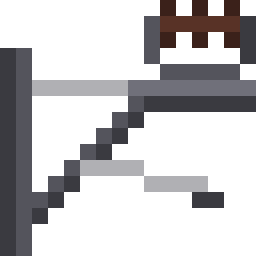
\includegraphics[width=1cm]{items/cantilever.png} & Iberian Cantilever & Create sequenced assembly from a PNW iron
rod bundle: two loops of deploying Iberian Steel, deploying a brown insulator and pressing. \\
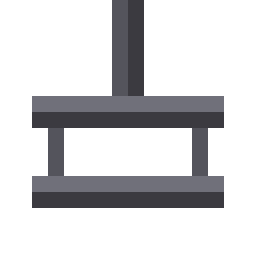
\includegraphics[width=1cm]{items/tunnel_support.png} & Iberian Tunnel Support & Two Iberian Steel above a brown
insulator; makes two. \\

\includegraphics[width=1cm]{items/rigid_profile.png} & Rigid Catenary Profile Bundle & Six Iberian Steel. \\
& Iberian masts & PNW iron strips with Iberian Steel (and iron rods for the square mast); six per craft. \\
& Iberian Pantograph & PNW pantograph and red dye (shapeless). \\
\bottomrule
\end{tabularx}
\end{center}

All recipes are visible in recipe viewers such as JEI, including the Create sequenced assembly.

% ---------------------------------------------------------------------------
\section{Technical summary}

\begin{center}
\begin{tabularx}{\linewidth}{@{}lX@{}}
\toprule
Minecraft & 1.20.1, Forge 47 \\
Required mods & Create: Pantographs \& Wires (1.20.1-beta-0.2.3-C6), Create 6.0.8, DragonLib, GeckoLib \\
License & GPL-3.0, the same as Pantographs \& Wires \\
Languages & English, Spanish, Catalan, German \\
Mod id & \texttt{iberiancantilever} \\
\bottomrule
\end{tabularx}
\end{center}

\paragraph{Integration with Pantographs \& Wires}
The add-on relies only on PNW's public building blocks: wire connectors, wire types registered in PNW's wire
registry and catenary graph, PNW's mast classes and tags, its pantograph and its GUI widgets. Its own content
(models, textures, translations and code) is self-contained, so it can be distributed as a separate add-on that
requires PNW, or merged into PNW as a set of additional blocks.

\paragraph{Credits}
\emph{Create: Pantographs \& Wires} by MrJulsen, on which this add-on is built, and \emph{Create} by the Create
team. Photographs from Wikimedia Commons, credited under each image and listed below.

\begin{footnotesize}
\begin{itemize}
  \item \emph{Catenaria Sant Adrià (Adif)} -- Adif -- Ineco, CC BY-SA 3.0.
        \url{https://commons.wikimedia.org/wiki/File:Catenaria_Sant_Adri%C3%A0_(Adif).jpg}
  \item \emph{Sant Adrià de Besòs station 2023 2} -- Smiley.toerist, CC BY-SA 4.0.
        \url{https://commons.wikimedia.org/wiki/File:Sant_Adri%C3%A0_de_Bes%C3%B2s_station_2023_2.jpg}
  \item \emph{J23 477 Bf Nules-La Villavieja} -- Falk2, CC BY-SA 4.0.
        \url{https://commons.wikimedia.org/wiki/File:J23_477_Bf_Nules-La_Villavieja.jpg}
  \item \emph{L04 380 Bf Valencia Fuente San Luis, Fahrleitungsstützpunkt} -- Falk2, CC BY-SA 4.0.
        \url{https://commons.wikimedia.org/wiki/File:L04_380_Bf_Valencia_Fuente_San_Luis,_Fahrleitungsst%C3%BCtzpunkt.jpg}
  \item \emph{Nuevos Ministerios L10 catenaria rígida} -- Draceane, CC BY-SA 4.0.
        \url{https://commons.wikimedia.org/wiki/File:Nuevos_Ministerios_L10_catenaria_rigida.jpg}
  \item \emph{Pantograph on top of Renfe Class 446 train at Córdoba} -- Philip Mallis, CC BY-SA 4.0.
        \url{https://commons.wikimedia.org/wiki/File:Pantograph_on_top_of_Renfe_Class_446_train_at_C%C3%B3rdoba_Julio_Anguita_Railway_Station_in_C%C3%B3rdoba,_Spain_(55066435535).jpg}
  \item \emph{S01 882 Stromabnehmer BR 449} -- Falk2, CC BY-SA 4.0.
        \url{https://commons.wikimedia.org/wiki/File:S01_882_Stromabnehmer_BR_449.jpg}
\end{itemize}
\end{footnotesize}

\end{document}
